\documentclass{article}
\usepackage{amsmath, amsthm, amssymb, bm, graphicx, mathrsfs, unicode-math}
\usepackage{hyperref} % content with links
\usepackage{bookmark, geometry}
\usepackage{listings, xcolor, caption, fancybox}

% add reference section. Must include at least one reference in the text.
\usepackage[nottoc]{tocbibind}
\usepackage[square,numbers]{natbib}
\bibliographystyle{abbrvnat}

\geometry{a4paper,scale=0.8}

\usepackage[english]{babel} % English formatting
\usepackage{fancyhdr} % Fancy headers
% \captionsetup[table]{position=bottom}
% \title{{\Huge{\textbf{Optimising MRI Pulse Sequence using Reinforcement Learning}}}\\\Huge{\textbf{PHAS0077}}\\\large{Outline}}
\title{\Huge{\textbf{Optimising MRI Pulse Sequence using Reinforcement Learning}}}
\author{Chongfeng Ling}
\date{\today}
\linespread{1}

%~~~~~~~~~ picture path
\graphicspath{{./assets}}

%~~~~~~~~~ Math theorem
\newtheorem{definition}{Definition}[section]
\newtheorem{remark}{Remark}[section]
\newtheorem{assumption}{Assumption}[section]
\newtheorem{theorem}{Theorem}[section]
\newtheorem{property}{Property}[section]

%~~~~~~~~~ Unknown scripts
\def\intinfty{\int_{-\infty}^{\infty}}
\renewcommand\thepart{\Alph{part}}

%~~~~~~~~~ short commands
\newcommand{\rr}{\mathbb{R}}
\newcommand{\refeq}[1]{Eq.\ref{#1}}
\newcommand{\pyobject}[1]{\ovalbox{\color{cyan}{\texttt{#1}}}}

%~~~~~~~~~ Listing
% New colors defined below
\definecolor{codegreen}{rgb}{0,0.6,0}
\definecolor{codegray}{rgb}{0.5,0.5,0.5}
\definecolor{codepurple}{rgb}{0.58,0,0.82}
\definecolor{backcolour}{rgb}{0.95,0.95,0.92}
% Code listing style
\lstdefinestyle{listing_style}{
  backgroundcolor=\color{backcolour},
  commentstyle=\color{codegreen},
  keywordstyle=\color{magenta},
  numberstyle=\tiny\color{codegray},
  stringstyle=\color{codepurple},
  basicstyle=\ttfamily\footnotesize,
  breakatwhitespace=false,         
  breaklines=true,                 
  captionpos=b,                    
  keepspaces=true,                 
  numbers=left,                    
  numbersep=5pt,                  
  showspaces=false,                
  showstringspaces=false,
  showtabs=false,                  
  tabsize=2
}
% Code listing set
\lstset{style=listing_style}
% rename name of "Listing"
\renewcommand\lstlistingname{Code}
\renewcommand\lstlistlistingname{Code}

%~~~~~~~~~ Page setup
\pagestyle{fancy}
\fancyhf{}
\lfoot{PHAS0077}
\rfoot{Page \thepage}
\renewcommand{\footrulewidth}{0.2pt}
\renewcommand{\headrulewidth}{0pt}

%~~~~~~~~~ Document start
\begin{document}

% center cover page
\null  % Empty line
\nointerlineskip  % No skip for prev line
\vfill
\let\snewpage \newpage
\let\newpage \relax
\maketitle
\setcounter{page}{0}
\thispagestyle{empty}
\let \newpage \snewpage
\vfill
\break % page break

%~~~~~~~~~ content page
\newpage
\pagenumbering{Roman}
\setcounter{page}{1}
\tableofcontents

%~~~~~~~~~ 
\newpage
\setcounter{page}{1}
\pagenumbering{arabic}

% \section{Purpose}
The Bloch equations provide a mathematical framework for characterizing the evolution of the magnetization over time. These equations describe the magnetization $B=(M_x, M_y, M_z)$ in terms of time $t$, the relaxation time $T_1$, $T_2$, and the external magnetic field $B$ and can be solved analytically with an explicitly defined pulse sequence. Though the Bloch equations play a crucial role in various applications of magnetic resonance imaging (MRI) and allow us to understand the behavior of the magnetization and obtain images, due to the nonlinear dynamics system they described, it is difficult to utilize the extensive parameters space in the pulse sequence to optimize our signal, especially when considering some physiological or technical limitations.
\\\\
Reinforcement Learning (RL) shows its huge potential in dealing with dynamic environments, particularly in areas such as gaming and autonomous systems (Chess and Go). It is a type of machine learning where an agent learns to make decisions by performing actions in an environment to maximize a reward signal. This approach allows the agent to learn from experience, adjusting its behavior over time to achieve the best results without knowing much about the action which have been used but simple rules.
\\\\
The main objective of this project is to optimizing MRI pulse sequence using Reinforcement Learning. Given a typical gradient-echo sequence-based signal, the goal is to design a new sequence that can produce an optimized signal under certain constraints including slew rate of a magnetization gradient field. A Python package will be released.

\section{Literature Review}

\citet{0477} presented a RL framework to solve the general design problem of pulse sequence. The target signal is obtained with a pre-defined pulse sequence and Bloch Equations under some constraints to meet experiment equipments and as showed in Figure.\ref{schematic}, the pulse sequence $X(t)$ is generated by a agent from a distribution $p(X)$. The distribution $p(X)$ is modeled by a dependent Gaussian process. The interaction between action $X(t)$ and environment is simulated by a Bayesian neural network $f:X(t) \rightarrow y$, where y is the score of the predicted signal compared with the target signal. To deal with the exploitation and exploration dilemma, the next set of pulse sequence $X^*$ is proposed by $p\left(f \mid y_t, X_{t+1}\right)$ by maximizing the acquisition function $u_t(X)$. They developed the MR physics simulator based on tool MRILAB. They performed the framework in 1-D experiments gradient echo with a fixed RF pulse, two simple constraints on $G_x$ is applied and gained a satisfied result. One year later they extended this framework to RF pulse design in 2-D experiments and showed the potentiality of the application of RL in pulse sequence design \cite{0438}.

\section{Methodology}

Our method will mainly follow the idea of the last two articles. The detailed implementation of algorithm will based on the MRILAB. The simulation of Bloch Equation with explicit gradient sequence has already been implemented in Python. This project will focus on designing 2-D Gradient Echo and after carrying out the algorithm implementation of the basic model, we will pay more attention on optimizing the slew rate of gradient.

\section{Challenge}

The foreseeable challenges of this project can be divided into several parts.
\\\\
Though the basic mechanism in MRI with pulse sequence has been taught in the related course, there is still a lot of relevant research that needs to be done, most notably to explore the constraints of mechanical properties on sequence design, in terms of performance and efficiency, in a realistic environment. In the current study, the main focus is on how to evaluate the slew rate and the effect of the overlap of two gradients on the output signal.
\\\\
This project involves the knowledge of Reinforcement Learning and Bayesian Neural Network that I had not learned before, so understanding and implementing the algorithms will be another major part of this project. Additionally, as our algorithm will involve huge matrix multiplication, optimizing our algorithms to reduce the running time in an acceptable time with a limited computational resources should be considered.

\begin{figure}[ht]
    \centering
    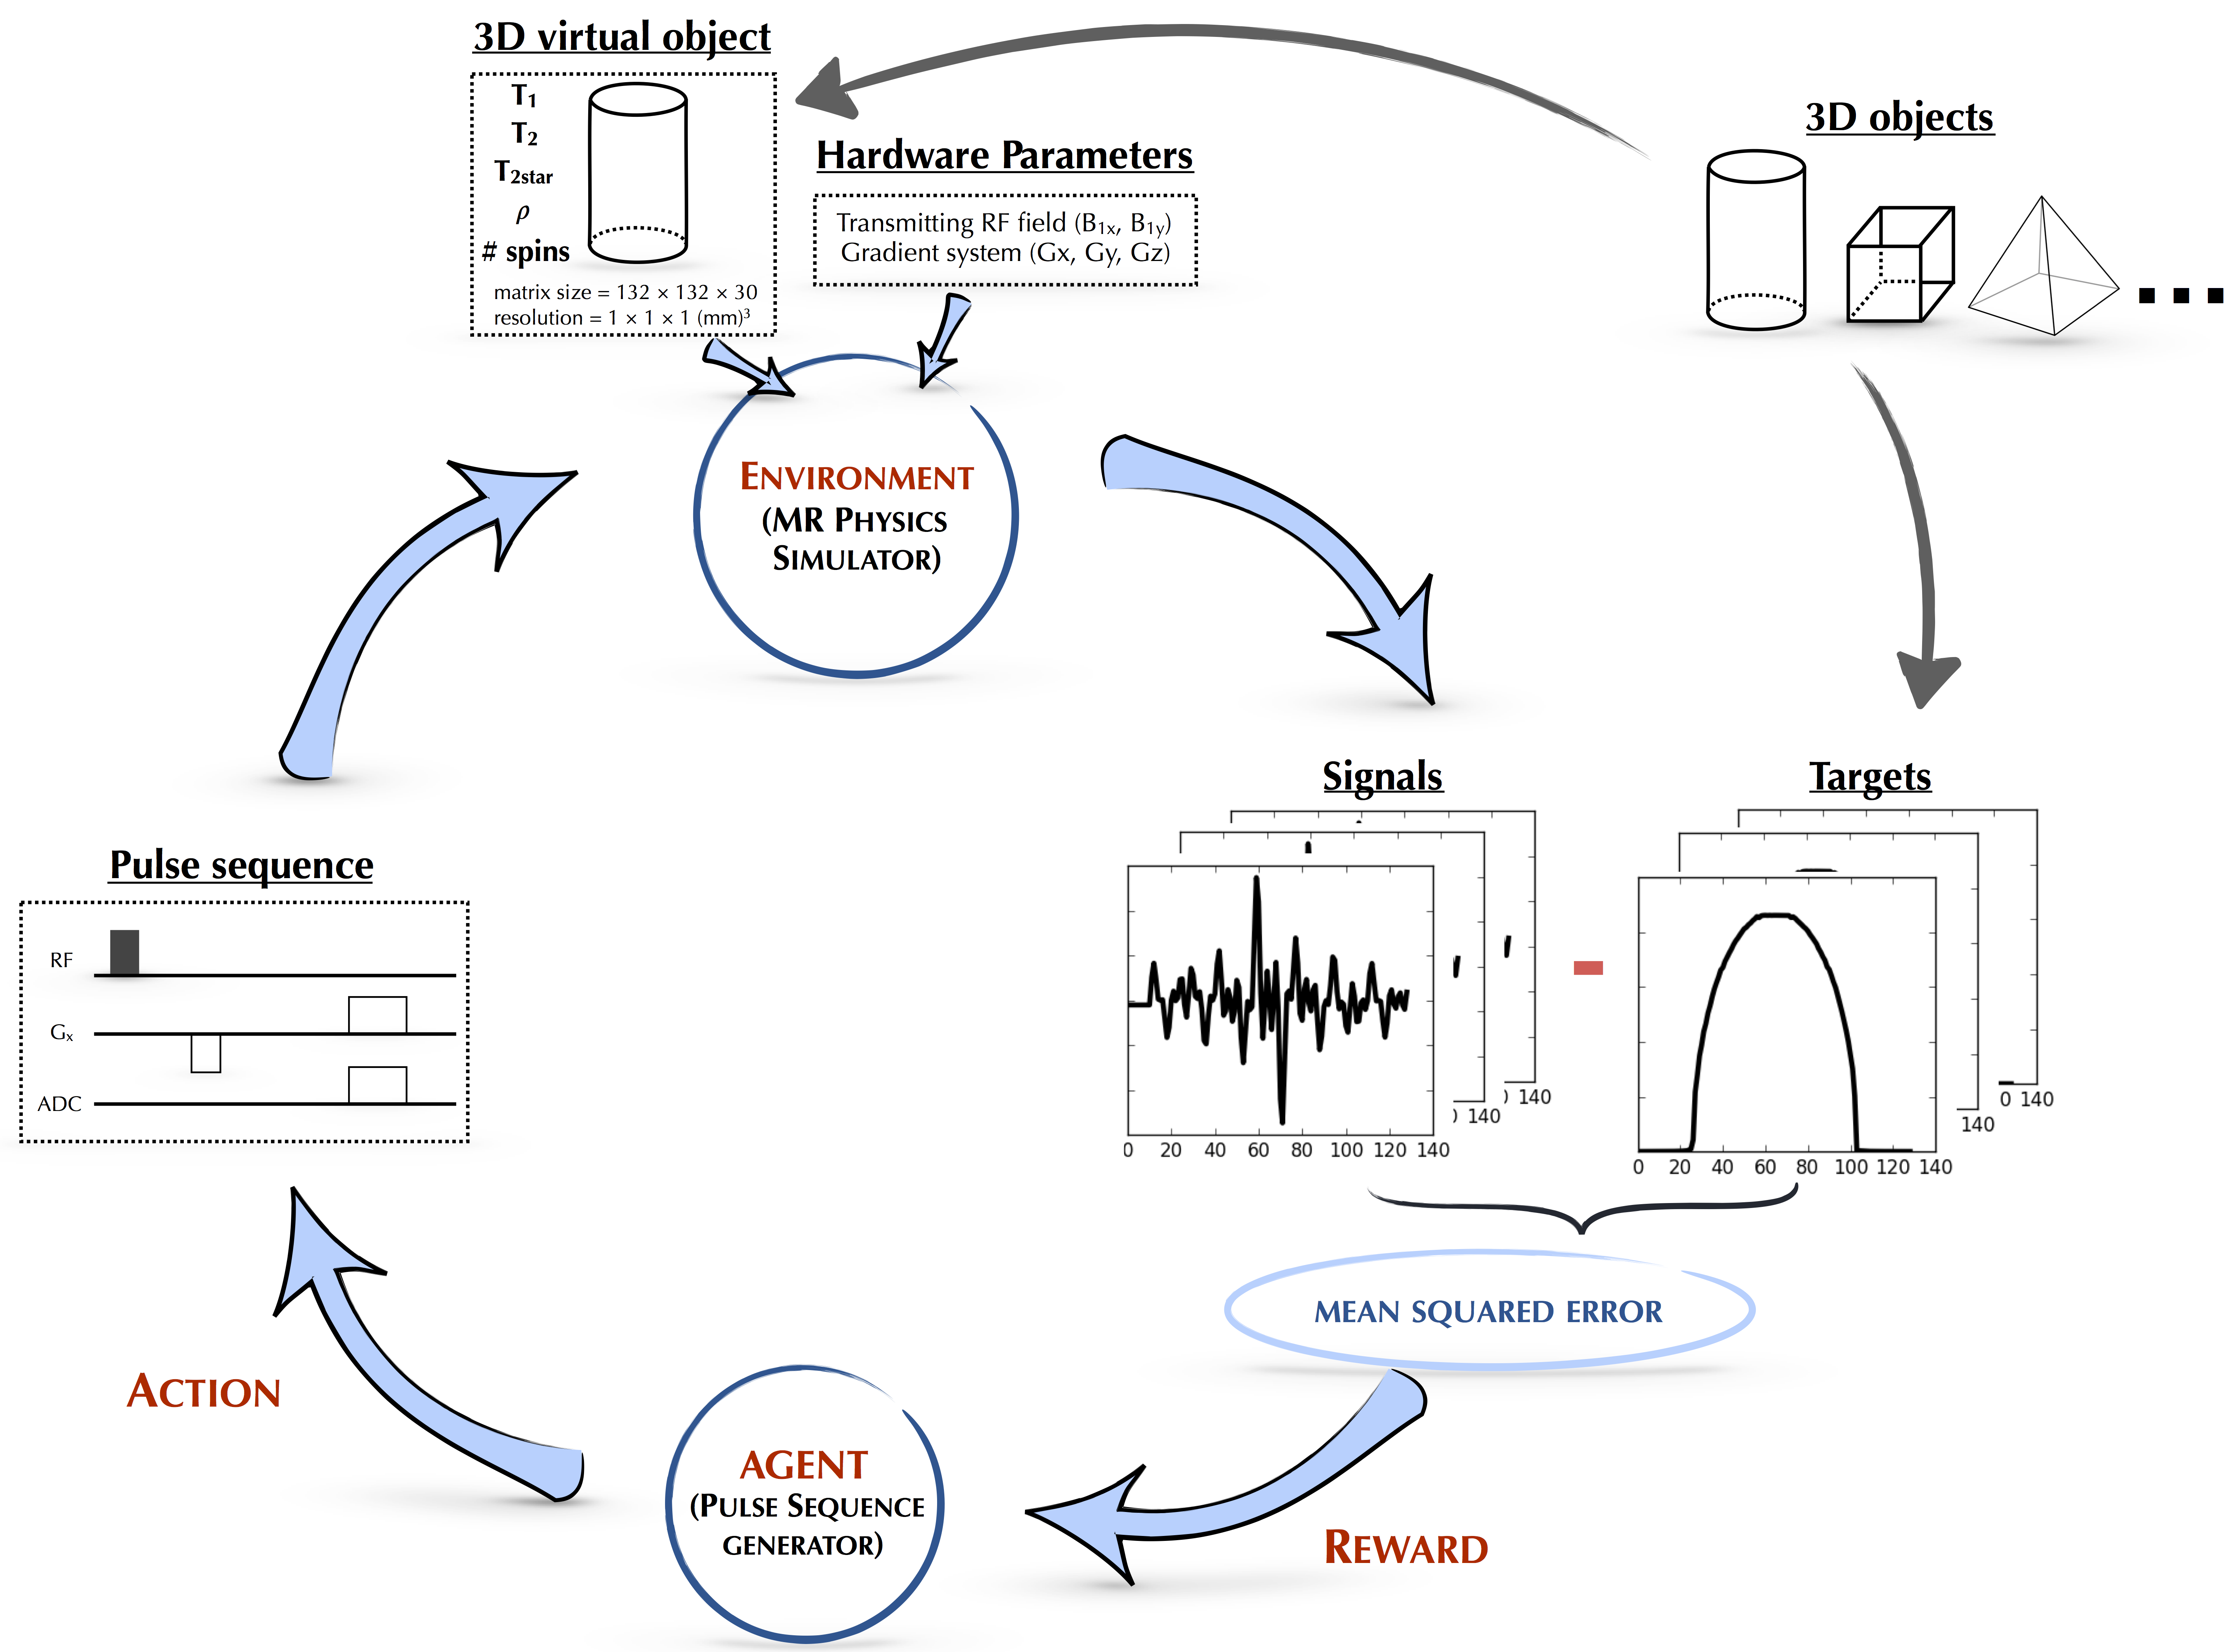
\includegraphics[scale=0.6]{schematic.png}
    \caption{title}
    \label{schematic}
\end{figure}
\section{Introduction and Problem Statement}
\subsection{What is the problem?}
Pulse sequences design in Magnetic Resonance Imaging (MRI) refers to the process of creating and optimizing a series of RadioFrequency (RF) pulses, magnetic field gradients and a static magnetic field to achieve a desired imaging goal. The interaction of these sequences manipulates the behavior of the nuclear spins in the body, which in turn produces a signal that can be used to form the basis of an image.

\subsection{Why is this problem important?}
The design of pulse sequences is a critical aspect of MRI, as it directly determines the quality of the image and acquisition time. Furthermore, the design of pulse sequences is various according to specific imaging applications and is constrained by the hardware and searching space of parameters \citep{0438}. Achieving a consistent and accurate image requires more than simply relying on default parameters. Instead, it necessitates the development of a model that takes into account the limitations of both the theoretical framework and realistic constraints involved in the imaging process.

\subsection{What is the goal of this project?}
The primary aim of this project is to create a Reinforcement Learning based model to optimize gradient echo sequence subject to some constraints. Specifically, the task involves designing a new pulse sequence generator that is capable of producing an optimized signal compared to a typical gradient-echo sequence-based signal, while conforming to certain constraints such as the slew rate of gradient coils.

\section{Literature Review}
\subsection{Existing relative researches and solutions}
Recent studies have incorporated the Reinforcement Learning framework to develop an optimal pulse sequence generator for obtaining consistent images compared to pre-designed pulse sequences. The research in this area can be broadly categorized into two primary segments: gradient echo (GE) sequence generator and radiofrequency wave (RF) generator, based on the sequence under consideration.
\\\\
As illustrated in Figure \ref{schematic}, \citet{0438} generated the gradient-echo sequence $X(t)$ by an agent from a distribution $p(X)$ that modeled by a dependent Gaussian process. The interaction between the action $X(t)$ and the environment was simulated by a Bayesian Neural Network $f:X(t) \rightarrow y$, where $y$ represented the score of the predicted signal compared with the target signal. To address the exploitation and exploration dilemma, the next predicted set of pulse sequences $X^*$ was proposed by $p\left(f \mid y_t, X_{t+1}\right)$ by maximizing the acquisition function $u_t(X)$.

\begin{figure}[ht]
    \centering
    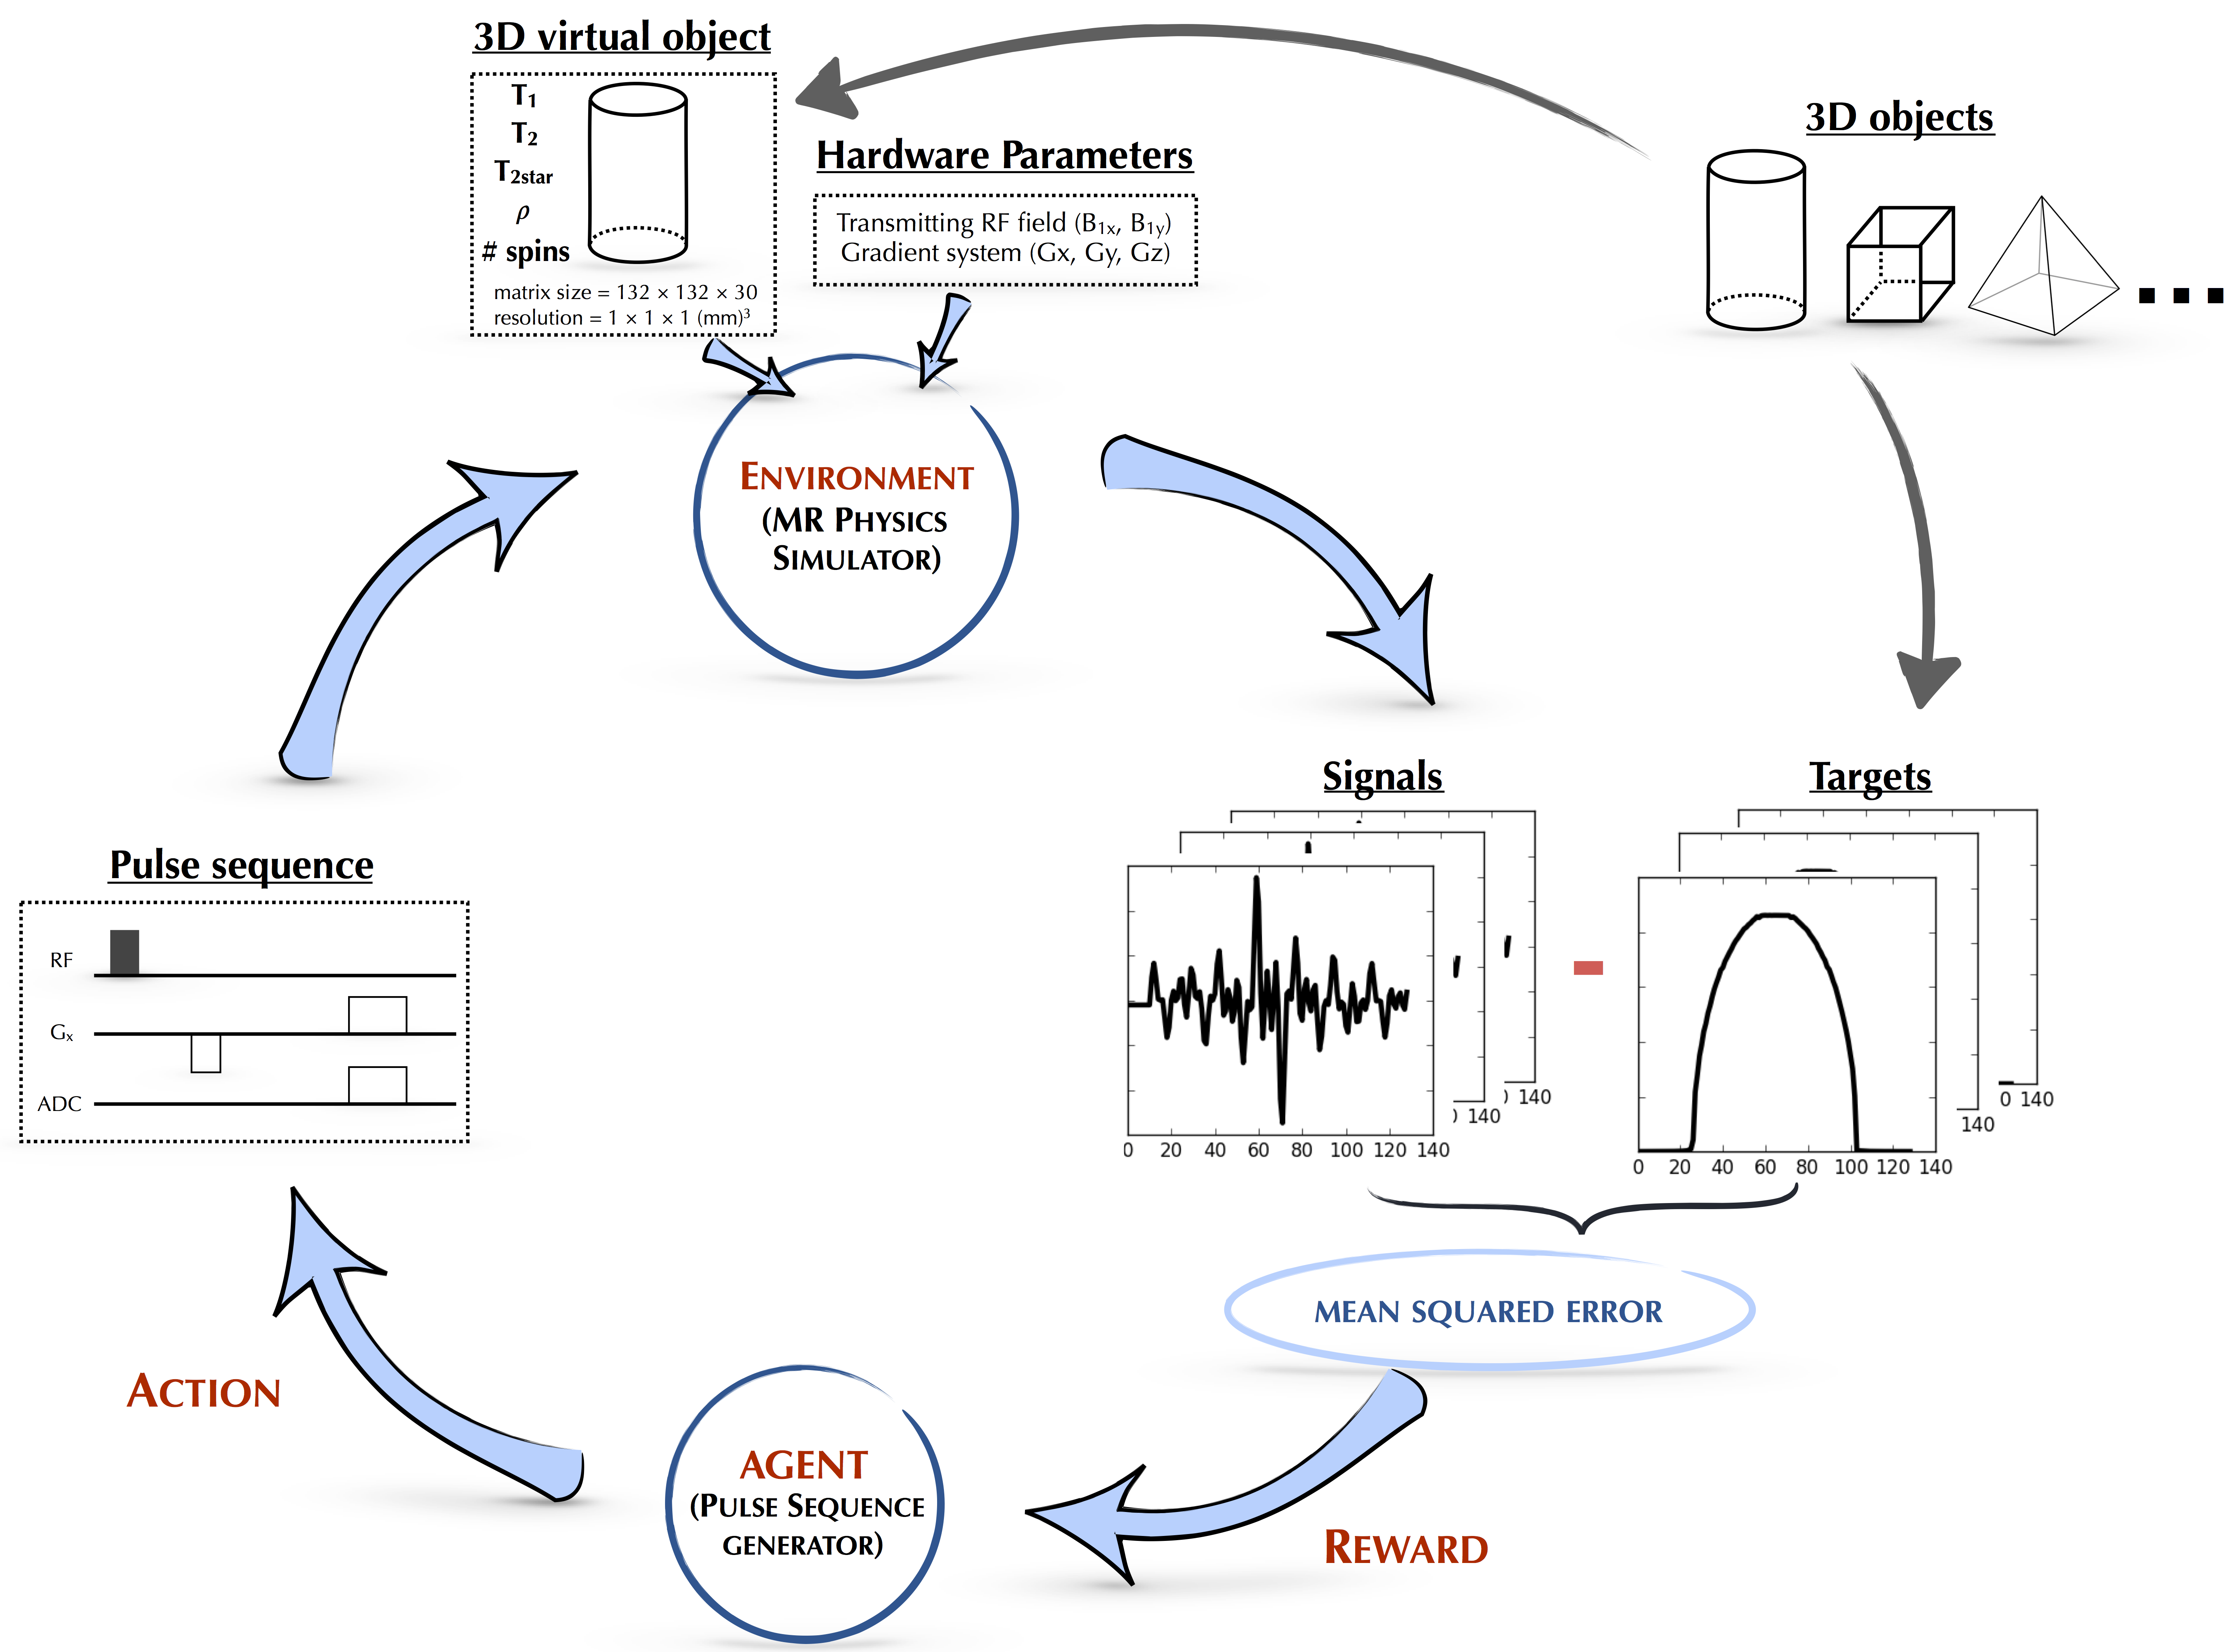
\includegraphics[scale=0.6]{schematic.png}
    \caption{Schematic of the AUTOSEQ Reinforcement Learning framework \citep{0438}.}
    \label{schematic}
\end{figure}

\subsection{Limitations of the current state of the art}
Though the preceding works have yielded satisfactory outcomes in addressing their respective problems, the empirical validation of the generalizability of RL models remains a critical concern. In an attempt to provide empirical evidence, \citet{0438} conducted experiments under a 1-D condition and examined specific constraints on a single $G_x$ but no conclusive evidence was presented regarding the generalizability of RL frameworks in more complex scenarios like higher dimensions or more sophisticated constraints. Additionally, a valuable research problem is the capacity to utilize the RL framework to design a comprehensive pulse sequence that encode radiofrequency (RF) waves and gradient echo sequences together.

\section{Methodology}

\subsection{Current baseline}

\subsection{Proposed method and its basis}


\section{Results and Analysis}

\subsection{Evaluation method}

\subsection{Results analysis}

\section{Plan and Challenges}


\bibliography{references}

\end{document}